%
% File naaclhlt2009.tex
%
% Contact: nasmith@cs.cmu.edu

\documentclass[11pt]{article}
\usepackage{naaclhlt2009}
\usepackage{times}
\usepackage{latexsym}
\usepackage[round]{natbib} 
\usepackage{amsmath}
\usepackage{amssymb} 
\usepackage[pdftex]{graphicx} 
\usepackage{hyperref} 
\usepackage{multirow}

\renewcommand{\baselinestretch}{.983} 

\setlength\titlebox{6.5cm}    % Expanding the titlebox

\title{Jointly Identifying Predicates, Arguments and Senses using Markov
Logic}

\author{
Ivan Meza-Ruiz$^{1}$ \\ {\tt I.V.Meza-Ruiz@sms.ed.ac.uk} \And Sebastian Riedel$^{2,3}$ \\ {\tt sebastian.riedel@gmail.com} \AND
${^1}$ {School of Informatics, University of Edinburgh, UK}\\
${^2}$ {Department of Computer Science, University of Tokyo, Japan}\\
${^3}$ {Database Center for Life Science, Research Organization of Information and System, Japan}\\
}

%SR: Fancy double affiliation for me :)

% \author{Ivan Meza-Ruiz \\
%   School of Informatics\\
%   University of Edinburgh, UK\\
%   {\tt I.V.Meza-Ruiz@sms.ed.ac.uk} \And
%   Sebastian Riedel\\
%   University of Tokio, Japan\\
%   {\tt S.R.Riedel@sms.ed.ac.uk}
%   }



\begin{document}

% Remember to aknowledge Mihai


\maketitle

%%% Local Variables: 
%%% mode: latex
%%% TeX-master: "paper"
%%% End: 

\newcommand{\R}{\mathcal{R}}
\newcommand{\T}{\mathcal{T}}
\newcommand{\bv}{\mathbf{v}}
\newcommand{\score}{s}
\newcommand{\obs}{\x_{o}}
\newcommand{\imp}{\Rightarrow}
\newcommand{\equi}{\Leftrightarrow}
\newcommand{\boldc}{\mathbf{c}}
\newcommand{\boldv}{\mathbf{v}}


\newcommand{\w}{\mathbf{w}}
\newcommand{\Y}{\mathcal{Y}}
\newcommand{\Yvar}{\mathbf{Y}}
\newcommand{\F}{F}
\newcommand{\opti}{\hat{\x}_{h}}
\newcommand{\f}{\mathbf{f}}
\newcommand{\x}{\mathbf{x}}
\newcommand{\y}{\mathbf{y}}
\newcommand{\ybest}{\hat{\y}}
\newcommand{\h}{\mathbf{h}}
\newcommand{\X}{\mathbf{X}}
\newcommand{\D}{\mathcal{D}}
\newcommand{\argmax}[1]{\underset{#1}{\text{arg max}}}
\newcommand{\guess}{\y'}
\newcommand{\Real}{\mathbb{R}}
\newcommand{\Int}{\mathbb{N}}
\newcommand{\bilevel}{\left\langle \Gamma,M\right\rangle }
\newcommand{\vocab}{\text{Vocabulary}}
\newcommand{\reduct}{\text{Reduct}}
\newcommand{\lforall}{\dot{\forall}}
\newcommand{\sscore}{\varsigma_{M}}
\newcommand{\cand}{\text{Cand}}
\newcommand{\unroll}{\text{Unroll}}
\newcommand{\ground}{\text{Ground}}
\newcommand{\mater}{\text{Materialize}}
\newcommand{\inner}{\text{Inner}}
\newcommand{\mapmodel}{\hat{N}}
\newcommand{\prob}{p}
\newcommand{\separate}{\text{Separate}}
\newcommand{\solve}{\text{solve}}
\newcommand{\MAP}{\text{MAP}}
\newcommand{\boldG}{\mathbf{G}}
\newcommand{\round}{\text{Round}}
\newcommand{\fracsolve}{\text{fractional-solve}}
\newcommand{\fractionals}{\text{Fractionals}}
\newcommand{\atoms}{\text{Atoms}}
\newcommand{\aux}{\lambda}
\newcommand{\smokes}{\forall x.\forall y.friends\left(x,y\right)\wedge smokes\left(x\right)\Rightarrow smokes\left(y\right)}
\newcommand{\data}{\mathcal{D}}
\newcommand{\I}{\mathbb{I}}
\newcommand{\Cliques}{\mathcal{C}}
\newcommand{\weightedsmokes}{\forall x.\forall y.\left(friends\left(x,y\right)\wedge smokes\left(x\right)\Rightarrow smokes\left(y\right)\left[w_{smokes}\right]\right)}
\newcommand{\ilpy}{\mathbf{a}}
\newcommand{\powerset}{\mathcal{P}}
\newcommand{\innersmokes}{friends\left(x,y\right)\wedge smokes\left(x\right)\Rightarrow smokes\left(y\right)}
\newcommand{\annasmokes}{smokes\left(Anna\right),friends\left(Anna,Peter\right)}
\newcommand{\finitevocab}{\left\{  \left\{  smokes,friends\right\}  ,\left\{  \right\}  ,\left\{  Anna,Peter\right\}  ,\left\{  x,y\right\}  \right\}  }
\newcommand{\determin}{\text{Deterministic}}
\newcommand{\nondeter}{\text{Nondeterministic}}


\begin{abstract}
In this paper we present a Markov Logic Network for Semantic Role
Labelling that jointly performs predicate identification, frame
disambiguation, argument identification and argument classification
for all predicates in a sentence. Empirically we find that our
approach is competitive: our best model would appear on par
with the best entry in the CoNLL 2008 shared task open track, and at
the 4th place of the closed track---right behind the systems that use
significantly better parsers to generate their input features.
%IV-
%In contrast, our model uses the vanilla MALT
%parses provided by the shared task organizers. 
Moreover, we observe
that by fully capturing the complete SRL pipeline in a single
probabilistic model we can achieve significant improvements over more isolated systems, in particular for out-of-domain
data. Finally, we show that despite the joint approach, our
system is still efficient. 
\end{abstract} 


\section{Introduction}


The search for the most likely translation (aka decoding, search,
MAP inference) given a statistical MT model has traditionally been
peformed by greedy or beam-based methods/heuristics {[}site some{]}.
While being efficient, most of these methods (do we know enough about
decoding to make any claims here?) have two drawbacks: (1) they are
approximate and give no bounds as to how far their solution is away
from the true optimum---this makes it sometimes hard to tell whether
the model or the search algorithm need to be improved; (2) they don't
scale (development-wise, not efficience) well with additional global
constraints. 

By constrast, recently researchers in other NLP appliciation areas
have increasingly relied on Integer Linear Programming as means to
find MAP solutions. ILP overcomes the two drawbacks mentioned above
as is guaranteed to be exact, and can be easily used to enforce global
constraints through additional linear inequalities. However, guaranteed
exactness, and generic global inference comes usually at the price
of efficiency. 

In fact, ILP has also been used as a method for MT decoding with IBM
Model 4 {[}cite Germann{]}. In {[}cite{]} work it became clear that
a naive ILP-based does not scale up to more than simple short sentences
due to an exponential number of constraints necessary to represent
the decoding problem in ILP. However, recent work in Dependency Parsing
{[}cite you and me{]} showed that ILP can still be efficient for very
large prograns when used in an incremental fashion. This raises the
question whether incremental/Cutting Plane ILP can also be used for
decoding of Model 4 for real world sentences. 

In this work we show that it is indeed possible to decode Model 4
with incremental ILP, at least for sentences to up to 30(? we have
to be more defensive here I think) words, and a simple two-gramm languange
model. This allowed us to give a definite answer as to how good/bad
Model 4 actually is, and how good/bad its state-of-the-art rewrite
decoder {[}cite{]}. Exact inference increases Bleu score by about
1 point for two language pairs when compared to the results of the
rewrite decoder {[}this is not really the answer{]}. From this we
conclude that the rewrite decoder indeed performs well, but still
can be slightly improved. (At the price of efficiency, that is)

Moreover, we believe that our work can be the basis of exciting and
really cool and also sexy future work. For example, as mentioned ILP
allows for a principled and declarative implementation of global constraints
and hence we may ask whether Model 4 can be improved through additional
global linguistic constraints; can we map other MT problems to an
ILP representation, and will this get slower, or maybe faster {[}why
could it{]}? How can larger language models be handled? (such models
are relatively easy to incorporate in left to right or greedy approaches
but pose a serious problem in the ILP sense). 

Finally, we observed that preprocessing and generating of ILPs is
as cpu-intensive as actual inference. This leads to the more general
question of how to integrate model construction more tightly with
the ILP solver (maybe by using Pricing strategies).

\section{Markov Logic} \label{sec:markovlogic}

Markov Logic (ML) \cite{richardson05markov} is a Statistical Relational Learning language based on First Order Logic and Markov Networks. It can be seen as a formalism that extends First Order Logic to allow formulae that can be violated
with some penalty. From an alternative point of view, it is an expressive
template language that uses First Order Logic formulae to instantiate
Markov Networks of repetitive structure. 

Let us describe Markov Logic by considering the predicate identification task. In Markov Logic we can model this task by first introducing a set of logical predicates\footnote{In the cases were is not obvious whether we refer to SRL or ML predicates we add the prefix SRL or ML, respectively.} such as \emph{isPredicate(Token)} or \emph{word(Token,Word)}. Then we specify a set of weighted first order formulae that define a distribution over sets of ground atoms of these predicates (or so-called \emph{possible worlds}). 

Ideally, the distribution we define with these weighted formulae assigns high probability to possible worlds where SRL predicates are correctly identified and a low probability to worlds where this is not the case. For example, a suitable set of weighted formulae would assign a high probability to the world\footnote{``Haag plays Elianti'' is a segment of a sentence in training corpus.}
\begin{eqnarray*}
 &\{ word\left(1,Haag\right),word(2,plays),\\
 & word(3,Elianti),isPredicate(2) \}& \end{eqnarray*}
and a low one to
\begin{eqnarray*}
& \{ word\left(1,Haag\right),word(2,plays),\\
 & word(3,Elianti),isPredicate(3) \} &\end{eqnarray*}
In Markov Logic a set $M=\left\{ \left(\phi,w_{\phi}\right)\right\} _{\phi}$ of weighted first order formulae is called a \emph{Markov Logic Network}~(MLN). It assigns the probability
\begin{equation}
\prob\left(\y\right)=\frac{1}{Z}\exp\left(
\sum_{\left(\phi,w\right)\in M} w
\sum_{\boldc\in C^{n_{\phi}}}f_{\boldc}^{\phi}\left(\y\right)
\right)
\label{eq:prob}
\end{equation}
to the possible world $\y$. Here $f_{\boldc}^{\phi}$ is a feature
function that returns 1 if in the possible world $\y$ the ground
formula we get by replacing the free variables in $\phi$ by the constants
in $\boldc$ is true and 0 otherwise. $C^{n_{\phi}}$ is the set
of all tuples of constants we can replace the free variables in $\phi$
with. $Z$ is a normalisation constant. Note that this distribution corresponds to a Markov Network where nodes represent ground atoms and factors represent ground formulae.

For example, if $M$ contains the formula $\phi$ \[
word\left(x,'take'\right)\Rightarrow isPredicate\left(x\right)\]
then its corresponding log-linear model has, among others, a feature 
$f_{t1}^{\phi}$ for which $x$ in $\phi$ has been replaced by the constant $t_1$ and that returns 1 if \[
word\left(1,'take'\right)\Rightarrow isPredicate\left(1\right)\]
is true in $\y$ and 0 otherwise.

We will refer predicates such as \emph{word} as \emph{observed} because they are known in advance. In contrast, \emph{isPredicate} is \emph{hidden} because we need to infer it at test time.




\section{Model} \label{sec:model} 



We define five hidden predicates for the three stages of the task. Figure \ref{fig:achitecture} illustrates these predicates and the stage they belong to. 
For predicate identification, we use the predicate \emph{isPredicate}. \emph{isPredicate(p)} indicates that the word in the position $p$ is an SRL predicate.

For argument identification and classification, we use the predicates \emph{isArgument}, \emph{hasRole} and \emph{role}. The atom \emph{isArgument(a)} signals that the word in the position $a$ is a SRL argument of some (unspecified) SRL predicate while \emph{hasRole(p,a)} indicates that the token at position $a$ is an argument of the predicate in position $p$. The predicate \emph{role(p,a,r)} corresponds to the decision that the argument in the position $a$ has the role $r$ with respect to the predicate in the position $p$.

Finally, for sense disambiguation we  define the predicate \emph{sense(p,e)} which signals that predicate in position $p$ has the sense $e$. 

\begin{figure}
\begin{center}
    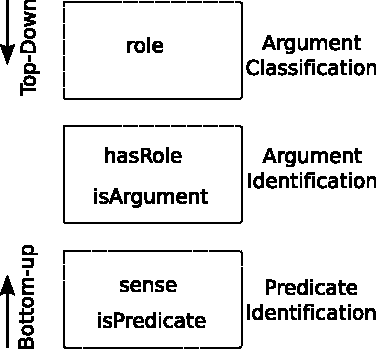
\includegraphics[scale=.70]{TaskArchitecture}
\end{center}
\caption{MLN hidden predicates divided in stages}
\label{fig:achitecture}
\end{figure}

\section{Local formulae}

A formula is local if its groundings relate any number of observed ground atoms to exactly one hidden ground atom. For example, a grounding of the local formula 
\[lemma(p,+l_1) \wedge lemma(a,+l_2) \Rightarrow hasRole(p,a)\]
can be seen in the Markov Network of Figure \ref{fig:local2}. It connects a hidden \emph{hasRole} ground atom to two observed \emph{lemma} ground atoms. Note that the ``+'' prefix for variables indicates that there is a different weight for each possible pair of lemmas $(l_1,l_2)$.

\begin{figure}
\begin{center}
    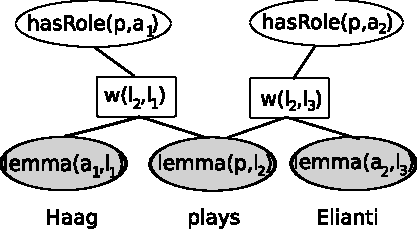
\includegraphics[scale=.70]{LocalFormula2}
\end{center}
\caption{Factor graph for the local formula in section \ref{sec:local}.}
\label{fig:local2}
\end{figure}

For the predicates \emph{isPredicate} and \emph{isArgument} we define the
following formuale:
\begin{description}
    \item[$Word$] a rule for the orthography of possible Predicate or Argument.
    \item[$Lemma_{-2,-1,1,2}$] for each lemma in a window of two previous and two following token a rule of possible Predicate or Argument.
    \item[$POSs_{-2,-1,1,2}$] for each POS in a window of two previous and two following tokens a rule of possible Predicate or Argument.
    \item[$CoarsePOS$] a rule for the previous and the following coarse POS tags of possible Predicate or Argument.
    \item[$CoarsePOS_2$] a rule for the two previous and two following corar POS tags of possible Predicate or Argument.
    \item[$DependecyChildren$] a rule for the dependencies of each child of possible Predicate or Argument.
    \item[$DependecyParent$] a rule for the dependencies of parent of possible Predicate or Argument.
    \item[$DependecyChildrenPOS$] a rule for the POS tag for each child  of possible Predicate or Argument.
    \item[$DependecyChildrenParPOS$] a rule for the POS tag of parent and each child  of possible Predicate or Argument.
    \item[$MFrame$] a rule for the MFrame of possible Predicate or Argument.
\end{description}



For the \emph{hasRole} and \emph{role} predicates we defined local formulae that aimed to reproduce the standard features used in previous work~\citep{xue04calibrating}. This also required us to develop dependency-based versions of the constituent-based features such as the syntactic path between predicate and argument, as proposed by \cite{xue04calibrating}. 

The remaining hidden predicates, \emph{isPredicate}, \emph{isArgument} and \emph{sense}, have local formulae that relate their ground atoms to properties of a contextual window around the token the atom corresponds to. For this we used the information provided in the closed track training corpus of the shared task (i.e. both versions of lemma and POS tags plus a coarse version of the POS tags). 




%Instead of describing the local feature set in more detail we refer the reader to our MLN model files.\footnote{\url{http://thebeast.googlecode.com/svn/mlns/conll08}} They can be used both as a reference and as input to our Markov Logic Engine\footnote{\url{http://thebeast.googlecode.com}}, and thus allow the reader to easily reproduce our results. We believe that this is another advantage of explicitly separating model and algorithms by using first order probabilistic logic languages.

\section{Global formulae}

\emph{Global} formulae relate several hidden ground atoms. We use them for two purposes: to ensure consistency between the decisions of all SRL stages and to capture some of our intuition about the task. We will refer to formulae that serve the first purpose as \emph{structural constraints}. 

% They aim to capture the relations between the hidden predicates, and ultimately of the stages of the SRL task. There are two types of global formulae: \emph{hard formulae} and \emph{soft formulae}. The hard formulae imposes constraints on the structure of the predicates. We can use hard formulae to solve the problem of coupling predicates.
For example, a structural constraint is given by the (deterministic) formula
\[role(p,a,r) \Rightarrow hasRole(p,a)\]
which ensures that, whenever the argument $a$ is given a label $r$ with respect to the predicate $p$, this argument must be an argument of $a$ as denoted by \emph{hasRole(p,a)}. Note that this formula by itself models the traditional ``bottom-up'' argument identification and classification pipeline: it is possible to not assign a role $r$ to an predicate-argument pair $(p,a)$ proposed by the identification stage; however, it is impossible to assign a role $r$ to token pairs $(p,a)$ that have not been proposed as potential arguments.

One example of another class of structural constraints is 
\[
hasRole(p,a)\Rightarrow\exists r.role(p,a,r)
\]
which, by itself, models an inverted or ``top-down'' pipeline. In this architecture the argument classification stage can assign roles to tokens that have not been proposed by the argument identification stage. However, it must assign a label to any token pair the previous stage proposes. 
%IV
Figure \ref{fig:global2} illustrates the structural formulae we use in form of a Markov Network.

The formulae we use to ensure consistency between the remaining hidden predicates are omitted for brevity as they are very similar to the bottom-up and top-down formulae we presented above.

For the SRL predicates that perform a labelling task (\emph{role} and \emph{sense}) we also need a structural constraint which ensures that not more than one label is assigned. For instance,
\[
(role(p,a,r_1) \wedge r_1 \neq r_2 \Rightarrow \neg role(p,a,r_2)  )
\]
forbids two different semantic roles for a pair of words. 

% thatrequires that for each \emph{hasRole} predicate there must be a SRL predicate in the postions $p$. This formula help us to relate two of the hidden predicates. The efect of the formula is similar to the bottom-up strategy where after identifing the the arguments of these are classified.

The global formulae that capture our intuition about the task itself can be further divided into two classes. The first one uses deterministic or \emph{hard} constraints such as
\begin{eqnarray*}
 &role\left(p,a_{1},r\right)\wedge \neg mod\left(r\right)\wedge a_{1}\neq a_{2}  \Rightarrow\\
  & \neg role\left(p,a_{2},r\right)
\end{eqnarray*}
which forbids cases where distinct arguments of a predicate have the same role unless the role describes a modifier.
%In this case we constrain to one semantic role to the words identify as proper arguments by the Palmer's heuristics. % ??

The second class of global formulae is \emph{soft} or nondeterministic. For instance, the formula  
\begin{eqnarray*}
  & lemma(p,+l) \wedge ppos(a,+p)  \\
  & \wedge hasRole(p,a)  \Rightarrow sense(p,+f) 
\end{eqnarray*}
is a soft global formula. It captures the observation that the sense of a verb or noun depends on the type of its arguments. Here the type of an argument token is represented by its POS tag.

%the relation between the \emph{hasRole} and \emph{sense} hidden predicates, together with the lemma of the SRL predicate and the POS tag of the argument. Figure \ref{fig:global2} is a graphical model representing the grounded version of this formula. %This formula does not imposes a structural constrain, but rather the link between the sense of the SRL predicate and its arguments.
%Why would this help?

\begin{figure}
\begin{center}
   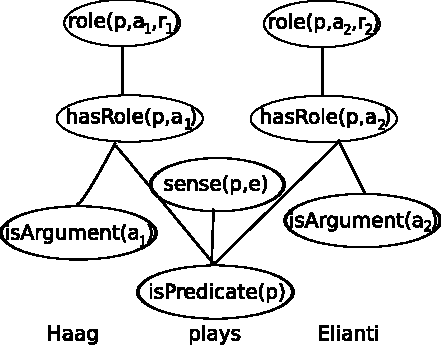
\includegraphics[scale=.70]{GlobalFormula2}
\end{center}
\caption{Markov Network that illustrates the structural constraints we use.}
\label{fig:global2}
\end{figure}






% Finally, to our last group of rules belongs the soft formulae and hard constrains with extra linguistic knowledge. Figure \ref{fig:global2} shows an example of soft formulae. An example, of hard constriain which uses extra linguistic knowledge is:
% \begin{eqnarray*}
%  & role\left(p,a_{1},r\right)\wedge arg\left(r\right)\wedge a_{1}\neq a_{2} & \Rightarrow\\
%   & \neg role\left(p,a_{2},r\right)
% \end{eqnarray*}
% In this case we constrain to one semantic role to the words identify as proper arguments by the Palmer's heuristics. % ??
%
%We have slit our global formulae into four groups. The first, are hard constrains which only involve one hidden predicate. The second one correspond to the hard constrains which involve more than one hidden predicate but follow a bottom-up strategy. This is conect two hidden predicates following the pipeline of the stages of the task. The top-down group group goes in a different direction. And finally, the fourth group contains the global formulae. In the section \ref{sec:results} we will explore how these relations contribute to the whole model. Table \ref{tbl:global} enumerate the global formulae used in this work.
%\begin{table}
%\begin{tabular}{|l|p{6cm}|}\hline
%Group & Description \\\hline
%1st   & There is one or less $role$ predicates for a pair of words (see Figure \ref{fig:hard1}.)\\
%      & There is one or less $frameLabel$ predicates for a word\\
%      & There are more than one $haslabel$ predicate for each word which is a possible argument by the Palmer heuristics\\\hline
%2nd   & If there is a $isPredicate(p)$ predicate, there must be a $frameLabel(p,_)$ predicate\\
%      & If thrre is a $isPredicate(p)$ predicate, there must be a $hasLabel(p,_)$ predicate\\      
%      & If there is a $hasLabel(p,a,_)$ predicate, there must be a $role(p,a,_)$ predicate\\\hline
%3rd   & If there is a $role(p,a,_)$ predicate, there must be a $hasLabel(p,a)$ predicate. \\
%      & If there is a $frameLabel(p,_)$ predicate, there must be a $isPredicate(p)$ predicate\\
%      & If there is a $hasLabel(p,_)$ predicate, there must be a $isPredicate(p)$ predicate.\\
%      & If there is a $hasLabel(_,a)$ predicate, there must be a $isArgument(a)$ predicate.\\\hline
%4th   & There shouldn't be two $hasLabel$ predicate for the which have as a predicate the same word, and the two arguments are prepositional phrases.\\
%      & There shouldn't be two predicates which overlap\\
%      & A $frameLabel$ predicated depends of the POS tags of the arguments of the predicate (see Figure \ref{fig:global1}\\
%      & For each proper argument defined by the Palmer heuristics there should be at most one $role$ predicate for that argument\\\hline
%      \end{tabular}
%\caption{Global formulae }
%\label{tbl:global}
%\end{table}
%




\section{Inference and Learning}\label{sec:inference}

%\subsection{Learning}

%An MLN we use to model the collective SRL task is presented in section \ref{sec:model}. We learn the weights associated this MLN using 1-best MIRA~\citep{crammer01ultraconservative} Online Learning method. 
%%Note that we only consider formulae that appear more than once in the training set.

%\subsection{Inference}

%%Assuming that we have an MLN with a set of suitable weights and a given sentence then we need to predict the choice of predicates, frame types, arguments and role labels with maximal a posteriori probability. To this end we apply a method that is both exact and efficient: Cutting Plane Inference~\citep[CPI,][]{riedel08improving} with Integer Linear Programming~(ILP) as base solver. We use it for inference at test time as well as during the MIRA online learning process.

Assuming that we have an MLN, a set of weights and a given sentence then we need to predict the choice of predicates, frame types, arguments and role labels with maximal a posteriori probability. To this end we apply a method that is both exact and efficient: Cutting Plane Inference~\cite[CPI,][]{riedel08improving} with Integer Linear Programming~(ILP) as base solver. We use it for inference at test time as well as during the MIRA online learning process.





\section{Experimental Setup}
\label{sec:experiments}

For our experiments we used a version of the CoNLL 2008 shared task~\citep{surdeanu08conll} dataset that only mentions verbial predicates, disregarding the nominal predicates available in the original corpus.\footnote{The reason for this choice is the fact that we could not get the license for the complete dataset.} While the original (open track) corpus came with MALT~\citep{nivre2007mli} dependencies, we observed slightly better results when using the dependency parses generated with a Charniak parser~\citep{charniak00amaximum}. Hence we used the latter for all our experiments.

%we modified the PropBank corpus of the CoNLL-05 shared task 
%\citep{carreras05introduction} to be compatible with the format of CoNL-08 
%shared task \citep{surdeanu08conll} which uses dependencies trees rather than 
%constituents. 
%IV+
%We choose to work with dependencies since recent development of dependency parsers had made possible for dependency-based SRL systems
%to reach state of the art performance \citep{johansson08dependency}. 
%We use the Charniak parses available in the original corpus and 
%converted into dependencies using the software developed by 
%\citet{johansson07conversion}. 

For our experimentation we create four systems. The first system, \emph{full model}, consists on the whole set of local and global formulae described in the previous section. 

In the second system, \emph{bottom-up} we eliminate the top-down structural constrains. This model simulates a  
pipeline system, in which decisions for ML predicates of the first statges have
stronger effect on the predicates of latter stages. However, this still is
joint model. 

Our third system, \emph{bottom-up (-isArg)}, departs from the second but it ommits the \emph{isArgument} hidden predicate and the formulae associated to it. With this modification this model follows a traditional approach where SRL system do not model the plausibility of a token of being argument.
% IV: Note, the results section says: this aspect of our model requires us to
% jointly perform inference for all predicates of a sentence. Dunno how to
% explain that.

Finally, the four system, \emph{pipeline}, is a pipeline system. In this case, we
create three models for each stage of our architecture (see Figure \ref{fig:achitecture}), and we pass the output of one as input of the next stage.


\section{Results}\label{sec:results}

In this section we describe our experimental setup and results.

\subsection{Experimental setup}
\label{sec:experimental-setup}

Our experimental setup is designed to answer several questions: (1) Is
exact inference in IBM Model 4 possible for sentences of moderate
length? (2) How fast is exact inference using the cutting plane
method? (3) How well does the ReWrite decoder perform in terms of
finding the optimal solution? (4) Does exact decoding increase provide
better translations?

In order to answer these questions we obtain a trained IBM Model 4 for
French-English and German-English on Europarl version 3 using GIZA++.
A bigram language model with Witten-Bell smoothing was built using the
CMU-Cambridge Language Modeling Toolkit.

For exact decoding we use the two models to generate ILP programs for
sentences of up to (and including) length 30 tokens for French and 25
tokens for German\footnote{These limits were imposed to ensure the
  Python script generating the ILP programs did not run out of
  memory.}.  We filter translation candidates in a similar manner to
(TODO:CITE) by using only the top ten translations for each
word\footnote{Based on $t(e|f)$.} and a list of zero fertility
words\footnote{Extracted using the rules in the filter script
  \texttt{rewrite.mkZeroFert.perl}}.  This resulted in 1101 French
sentences and 1062 German sentences for testing purposes.  The ILP
programs were then solved using the method described in
Section~\ref{sec:ilp}.  The same models were used with the ISI ReWrite
Decoder to solve the same set of sentences.


\subsection{Results}
\label{sec:results-results}

\begin{table*}[t]
  \centering
  \subfloat[French-English\label{tab:results:french}] {
    \footnotesize
  \centering
  \begin{tabular}{|l|r|r|r|r|r|r|r|r|}
    \hline
    \multirow{2}{*}{Length} & \multirow{2}{*}{\#} & \multicolumn{4}{|c|}{Solve Stats} & \multicolumn{3}{|c|}{BLEU} \\
    & & \% eq & \% gt & \%err & ST & ReW & ILP & Diff \\
    \hline
    1--5   & 21  & 52.4 & 47.6 & 6.9 & 0.7   & 56.47 & 56.15 &-0.32  \\
    6--10  & 121 & 47.9 & 52.1 & 5.2 & 1.4   & 26.11 & 28.01 & 1.90  \\
    11--15 & 118 & 37.2 & 62.8 & 3.2 & 2.7   & 22.85 & 23.70 & 0.85  \\
    16--20 & 238 & 32.4 & 67.6 & 3.2 & 13.9  & 20.40 & 20.81 & 0.41  \\
    21--25 & 266 & 25.2 & 74.8 & 3.1 & 70.1  & 20.89 & 22.51 & 1.62  \\
    26--30 & 152 & 22.4 & 77.6 & 2.4 & 162.6 & 20.92 & 22.30 & 1.38  \\
    \hline                                    
    1--30  & 986 & 32.1 & 67.9 & 3.3 & 48.1  & 21.66 & 22.63 & 0.97  \\
    \hline
  \end{tabular}
}\\
\subfloat[German-English\label{tab:results:german}] {
  \centering
  \footnotesize
  \begin{tabular}{|l|r|r|r|r|r|r|r|r|}
    \hline
    \multirow{2}{*}{Length} & \multirow{2}{*}{\#} & \multicolumn{4}{|c|}{Solve Stats} & \multicolumn{3}{|c|}{BLEU} \\
    & & \% eq & \% gt & \% err & ST & ReW & ILP & Diff \\
    \hline
    1--5   & 31  & 0.0 & 100.0 & 8.3 & 0.8   & 40.68 & 41.12 & 0.44  \\
    6--10  & 175 & 0.0 & 100.0 & 6.2 & 1.7   & 19.19 & 20.91 & 1.72  \\
    11--15 & 242 & 0.0 & 100.0 & 5.3 & 5.5   & 15.97 & 16.69 & 0.72  \\
    16--20 & 257 & 0.0 & 100.0 & 4.4 & 23.9  & 15.78 & 15.94 & 0.16  \\
    21--25 & 249 & 0.0 & 100.0 & 4.2 & 173.4 & 15.31 & 15.92 & 0.61  \\
    \hline                                   
    1--25  & 954 & 0.0 & 100.0 & 5.0 & 53.5  & 16.10 & 16.71 & 0.61   \\
    \hline
  \end{tabular}
}
\caption{\footnotesize Results on the two corpora.  Length: range of sentence lengths; \#: number of sentences in this range; \% eq: percentage of times ReWrite decoder and ILP decoder returned same model score; \% gt: percentage of times ILP decoder returned higher result than ReWrite; \% err: the micro-averaged percentage error between log model scores; ST: the average solve time per sentence of ILP decoder in seconds; BLEU ReW, BLEU ILP, BLEU Diff: the BLEU scores of the output and difference between BLEU scores.}  \label{tab:comparison}
\end{table*}

% TODO: difficult to decide how strong our claims can be regarding is
% ILP-M4 possible?
The ILP decoder produced output for 986 French sentences and 954
German sentences.  From this we can conclude that it is possible to
solve 90\% of our sentences exactly using ILP.  For the remaining 115
and 108 sentences we did not produce a solution due to: (1) the solver
not completing within 30 minutes, (2) the solver running out of
memory, or (3) the solver producing a one word output due to
(TODO:INSERT EXPLANATION).

Table~1 shows a comparison of the results obtained on the 986 French
and 954 German sentences using the ILP and ReWrite decoders.  The
results are broken down by sentence length range of the input
sentence.  We now turn our attention to the solve times obtained using
ILP (for the sentences for which the solution was found 30 minutes).
The table shows that the average solve time if under a minute per
sentence.  This longer sentences taking on average more time.  Thus
using the cutting planes method with ILP makes solving the ILP
programs tractable in practice (TODO: Really?).

% TODO: This next paragraph is strange, the percentage error in log
% space is strange in general!  And it is kind of out of the blue.
We next examine the model scores.  We can see in the French case the
ReWrite decoder finds the optimal solution 32.1\% of the time for
French and 0\% for German.  Although the same English string is
produced for 40.1\% of the French sentences and 29.1\% of the German
sentences\footnote{There may be precision and rounding errors in
  comparing the model scores, we call two log model scores equal if
  they are within 0.1 of one another}.  The percentage error rate
indicates how far away the ReWrite decoder's solution was from the
optimal in terms of log model score\footnote{We consider the
  percentage error of log scores because the numbers involved when
  converted to probabilities are very small resulting in large
  percentage errors.  Approximate macro-averaged percentage error of
  60\% for both corpora.}.  This number is a little misleading
although the percentage error rate is decreasing for longer sentences
in log space it is actually increasing in probability error space.  It
is difficult to interpret these percentage errors in either log space
or probability space.

Performing exact decoding increases the BLEU score by 0.97 points on
the French-English data set and 0.61 points on the German-English data
set.



% General averages:
% French: 
% 32.1\% of the time ReWrite and ILP equal in model score.
% 67.9\% of the time ILP beats ReWrite in model score.
% Log space stats:
% Micro averaged percentage error: 3.3\% (similar for macro)
% Maximum percentage error: 22.0\%
% Minimum percentage error (on the 67.1\%):  0.1\%
% Probability space stats:
% Micro averaged percentage error: 82.2\%
% Macro averaged percentage error: 60.6\%
% Maximum percentage error: 100.0\%
% Minimum percentage error: 21.5\%

% German: 
% 100\% of the time ILP beats ReWrite in model score.
% Log space stats:
% Micro averaged percentage error: 5.0\% (similar for macro)
% Maximum percentage error: 65.0\%
% Minimum percentage error:  0.7\%
% Probability space stats:
% Micro averaged percentage error: 95.3\%
% Macro averaged percentage error: 60.9\%
% Maximum percentage error: 100.0\%
% Minimum percentage error: 52.6\%



% \begin{table}[tp]
%   \centering
%   \begin{tabular}{|c|l|l|l|l|}
%     \hline
%     Length & Count & \%eq & \%R$<$ILP & Av.\%err \\
%     \hline
%     1--5 & 21 & 52.4 & 47.6 & 6.9 \\
%     6--10 & 121 & 47.9 & 52.1 & 5.2 \\
%     11--15 & 118 & 37.2 & 62.8 & 3.2 \\
%     16--20 & 238 & 32.4 & 67.6 & 3.2 \\
%     21--25 & 266 & 25.2 & 74.8 & 3.1 \\
%     26--30 & 152 & 22.4 & 77.6 & 2.4 \\
%     \hline 
%     1--30 & 986 & 32.1 & 67.9 & 3.3 \\
%     \hline
%   \end{tabular}
%   \caption{French comparisons}
%   \label{tab:french-compare}
% \end{table}

% \begin{table}[tp]
%   \centering
%   \begin{tabular}{|c|l|l|l|l|}
%     \hline
%     Length & Count & \%eq & \%R$<$ILP & Av.\%err \\
%     \hline
%     1--5 & 31 & 0.0 & 100.0 & 8.3 \\
%     6--10 & 175 & 0.0 & 100.0 & 6.2 \\
%     11--15 & 242 & 0.0 & 100.0 & 5.3 \\
%     16--20 & 257 & 0.0 & 100.0 & 4.4 \\
%     21--25 & 249 & 0.0 & 100.0 & 4.2 \\
%     \hline 
%     1--25 & 954 & 0.0 & 100.0 & 5.0 \\
%     \hline
%   \end{tabular}
%   \caption{German comparisons}
%   \label{tab:german-compare}
% \end{table}

% Length - length range of sentence (inclusive).
% Count - number of sentences in this length range.
% \%eq - percentage of time outputs had equal log model score (precision 0.1)
% \%R$<$ILP - percentage of time ILP had higher log model score than ReWrite.
% Av. \%err - average percentage error between the log model scores

% \begin{table}[tp]
%   \centering
%   \begin{tabular}{|c|l|l|l|l|}
%     \hline
%     Length & ReWrite BLEU & ILP BLEU & Diff & ILP ST \\
%     \hline
%     1--5 & 56.47 & 56.15 & -0.32 & 0.7 \\
%     6--10 & 26.11 & 28.01 & 1.90 & 1.4 \\
%     11--15 & 22.85 & 23.70 & 0.85 & 2.7 \\
%     16--20 & 20.40 & 20.81 & 0.41 & 13.9 \\
%     21--25 & 20.89 & 22.51 & 1.62 & 70.1 \\
%     26-30 & 20.92 & 22.30 & 1.38 & 162.6 \\
%     \hline 
%     1--30 & 21.66 & 22.63 & 0.97 & 48.1 \\
%     \hline
%   \end{tabular}
%   \caption{French Analysis}
%   \label{tab:french-analysis}
% \end{table}

% \begin{table}[tp]
%   \centering
%   \begin{tabular}{|c|l|l|l|l|}
%     \hline
%     Length & ReWrite BLEU & ILP BLEU & Diff & ILP ST \\
%     \hline
%     1--5 & 40.68 & 41.12 & 0.44 & 0.8 \\
%     6--10 & 19.19 & 20.91 & 1.72 & 1.7 \\
%     11--15 & 15.97 & 16.69 & 0.72 & 5.5 \\
%     16--20 & 15.78 & 15.94 & 0.16 & 23.9 \\
%     21--25 & 15.31 & 15.92 & 0.61 & 173.4 \\
%     \hline 
%     1--25 & 16.10 & 16.71 & 0.61 & 53.5 \\
%     \hline
%   \end{tabular}
%   \caption{German Analysis}
%   \label{tab:german-analysis}
% \end{table}

% Diff - BLEU difference between ILP and ReWrite
% ILP ST - average ILP solve time per sentence in seconds.



%%% Local Variables: 
%%% mode: latex
%%% TeX-master: "ilp-mt"
%%% End: 


\section{Conclusion} \label{sec:conclusion}

In this paper we have demonstrated that optimal decoding of IBM Model
4 is more practical than previously suggested.  Our results and
analysis show that exact decoding has a practical purpose.  It has
allowed us to investigate and validate the performance of the ReWrite
decoder through comparison of the outputs and model scores from the
two decoders.  Exact inference also provides an improvement in
translation quality as measured by BLEU score.

During the course of this research we have encountered numerous
challenges that were not apparent at the start.  These challenges
raise some interesting research questions and practical issues one
must consider when embarking on exact inference using ILP.  The first
issue is that the generation of the ILP programs can take a long time.
This leads us to wonder if there may be a way to provide tighter
integration of program generation and solving.  Such an integration
would avoid the need to query the models in advance for \emph{all}
possible model components the solver may require.

Related to this issue is how to tackle the incorporation of higher
order language models. Currently we use our bigram language model in a
brute-force manner: in order to generate the ILP we evaluate the
probability of all possible bigrams of English candidate tokens in
advance. It seems clear that with higher order models this process
will become prohibitively expensive. Moreover, even if the ILP could
be generated efficiently, they will obviously be larger and harder to
solve than our current ILPs. One possible solution may be the use of
so-called delayed column generation strategies which incrementally add
parts of the objective function (and hence the language model), but
only when required by the ILP solver.\footnote{Note that delayed
  column generation is dual to performing cutting planes.}

The use of ILP in other NLP tasks has provided a principled and
declarative manner to incorporate global linguistic constraints on the
system output.  This work lays the foundations for incorporating
similar global constraints for translation.  We are currently
investigating linguistic constraints for IBM Model~4 and other
word-based models in general.  A further extension is to reformulate
higher-level MT models (phrase- and syntax-based) within the ILP
framework.  These representations could be more desirable from a
linguistic constraint perspective as the formulation of constraints
may be more intuitive.


%%% Local Variables: 
%%% mode: latex
%%% TeX-master: "ilp-mt"
%%% End: 


\section*{Acknowledgment}

The authors are grateful to Mihai Surdeanu for providing the version of
the PropBank corpus used in this work.

\bibliographystyle{plainnat}
\bibliography{seb}


\end{document}

% Comments
%---
% Reviewer 1
%---
% 1. error analysis can be very difficul, discussed.
%    IV. Mention this ??
% 2. The natural question, why the authors didn't switch parsers.
%    IV. Dogde this ball, for now.
% 3. Statistical signficant.
%    IV. Maybe do this
% 4. Number of assigments
%    IV. ?? No idea what's this.
% 5. Pipe-line -> other systems.
%    IV. Make clear this is seb's implementation (include beast links and models)
% 6. Equation (1), w is the same as w-sub-phii next line? 
%    I think it should be the same, check with Seb
% 7. Phi Subscript for (phi,w), is it right?
%    I think it is right
% 8. primes x' and take'.
%    Erase the simple quotes (Done)
% 9. Figure 2, functor w?
%    Figure says rectangles are formulae and functors. We need to clarify this.
%    (done)
% 10. Figure 2, subscript a, rather than a simple index.
%    Change the subscripts.
% 11. Explanation of '+'
%     Imply that weights have indeces, rather than what means. (done)
% 12. End of Section 1.  Second reference to section 3 looks like it should be to
%     section 4.
 
 
%---
% Reviewer 2
%---
% 1. For comparison purposes, are better parses available?
%    IV. Dodge the ball.
% 2. If so, would using them result in significantly different results?
%    IV. Maybe hint this happens, otherwise dodge the ball.
% 3. high-level description of previously published inference methods -
%    I'd suggest either including some lines of pseudocode or just including the pointers to the previous work - right now.
% 4. which contains not just an interpreter but also a number of inference algorithms ?)
%    Alchemy

%---
% Reviewer 3
%============================================================================
                            %REVIEWER #3
%============================================================================ 

% 1. little more detail in the particulars of the MLN training process,i
% 2. how the data was prepared in order for used as input.

